% Using Free and Open Source Solutions in Geospatial Science Education
% This work by Vaclav Petras is licensed under
% a Creative Commons Attribution-ShareAlike 4.0 International License.

\documentclass[xcolor={dvipsnames,usenames},beamer,aspectratio=169]{beamer}
% ,handout,notes=show

\makeatletter
\def\beamer@framenotesbegin{% at beginning of slide
  \gdef\beamer@noteitems{}%
  \gdef\beamer@notes{{}}% used to be totally empty.
}
\makeatother

\usepackage{textcomp}
\usepackage[utf8]{inputenc}
\usepackage[american]{babel}
\usepackage{graphicx}
\usepackage{url}
\usepackage{amssymb}

\usepackage{tikz}
\usetikzlibrary{arrows,shapes,spy,calc}

\tikzstyle{every picture}+=[remember picture]
\tikzstyle{na} = [baseline=-.5ex]

% frames have to be fragile
\newif\ifnotes
% \input{tmpnotessettings}
% \notestrue


\ifnotes
\setbeamertemplate{note page}[plain]
% \setbeamertemplate{note page}[compress]
\setbeamerfont{note page}{size=\large}
% \setbeameroption{show only notes}
\setbeameroption{show notes}
\usepackage{pgfpages}
\pgfpagesuselayout{2 on 1}[a4paper,border shrink=5mm]%
\else
%\setbeameroption{hide notes}
\fi
%\notesfalse

\usepackage[absolute,overlay]{textpos}

\usepackage{listings}


% \usetheme{Warsaw}
\usetheme{Madrid}
% \usetheme{Frankfurt}
% \useoutertheme{infolines}
\usecolortheme[named=MidnightBlue]{structure}
% \usecolortheme[named=PineGreen]{structure}
\setbeamertemplate{navigation symbols}{}

\setbeamertemplate{itemize items}[default]
\setbeamertemplate{enumerate items}[default]
% \useinnertheme{rectangles}
\setbeamertemplate{blocks}[default]


%%%%%%%%%%%%%%%%%%%%%%%%%%%%%%%%%%%%%%%%%%%%%%%%%%%%%%%%%%%%%%%%%%%%
%%%%%%%%%%%%%%%%%%%%%%%%%%%%%%%%%%%%%%%%%%%%%%%%%%%%%%%%%%%%%%%%%%%%

% \newcommand{\n}[1]{$^{\color{gray}{\mbox{\tiny#1}}}$}
\newcommand{\n}[1]{$^{\textcolor{gray}{\mbox{\tiny #1}}}$}

%%%%%%%%%%%%%%%%%%%%%%%%%%%%%%%%%%%%%%%%%%%%%%%%%%%%%%%%%%%%%%%%%%%%%%%%%%%%%%%
\newcommand{\gmodule}[1]{\href{http://grass.osgeo.org/grass71/manuals/#1.html}{\emph{#1}}}
\newcommand{\amodule}[1]{\href{http://grass.osgeo.org/grass70/manuals/addons/#1.html}{\emph{#1}}}
\newcommand{\module}[1]{\emph{#1}}
\newcommand{\grasslink}{\href{http://grass.osgeo.org/}{GRASS GIS}}

%%%%%%%%%%%%%%%%%%%%%%%%%%%%%%%%%%%%%%%%%%%%%%%%%%%%%%%%%%%%%%%%%%%%
%%%%%%%%%%%%%%%%%%%%%%%%%%%%%%%%%%%%%%%%%%%%%%%%%%%%%%%%%%%%%%%%%%%%

\title[Processing of point clouds in GRASS GIS]
{Efficient processing of dense point clouds in GRASS GIS}
\subtitle{at US-IALE 2016 Annual Meeting}
%\pdforstring{}{}

\author[Vaclav Petras]
{Vaclav Petras (Vashek)\\%\n{1,2}\\
{
\scriptsize
Douglas Newcomb, %\n{3},
%\mbox{
Helena Mitasova%\n{1,2}
%}
}
}

\institute[NC State University]
{%
Center for Geospatial Analytics
% \tiny
%\n{1}NCSU Department of Marine, Earth and Atmospheric Sciences \\
%\n{2}NCSU Center for Geospatial Analytics \\
%\n{3}U.S. Fish and Wildlife Service

\bigskip

\includegraphics[width=0.3\textwidth]{logos/ncstate}
}

\date{March 18, 2016}

\setbeamercovered{transparent}

\hypersetup{%
 pdfauthor={Vaclav Petras},%
 pdfsubject={GRASS GIS and lidar talk at US-IALE 2016},%
 pdfkeywords={UAV} {UAS} {point clouds} {lidar}
   {v.in.lidar} {r.in.lidar} {v.decimate} {v.out.lidar} {libLAS}
   {geospatial modeling} {GRASS GIS}
   {free software} {open source} {open science}
}

\usepackage{tipa}
\newcommand{\pron}[2]{#1 [#2]}


\newcommand{\beginbackup}{
  \newcounter{framenumbervorappendix}
  \setcounter{framenumbervorappendix}{\value{framenumber}}
}
\newcommand{\backupend}{
  \addtocounter{framenumbervorappendix}{-\value{framenumber}}
  \addtocounter{framenumber}{\value{framenumbervorappendix}}
}


%%%%%%%%%%%%%%%%%%%%%%%%%%%%%%%%%%%%%%%%%%%%%%%%%%%%%%%%%%%%%%%%%%%%
% when images are placed in these directories, we don't have to specify the directory
% just the filename
\graphicspath{{img/}{figures/}{images/}}


%%%%%%%%%%%%%%%%%%%%%%%%%%%%%%%%%%%%%%%%%%%%%%%%%%%%%%%%%%%%%%%%%%%%
%%%%%%%%%%%%%%%%%%%%%%%%%%%%%%%%%%%%%%%%%%%%%%%%%%%%%%%%%%%%%%%%%%%%
%%%%%%%%%%%%%%%%%%%%%%%%%%%%%%%%%%%%%%%%%%%%%%%%%%%%%%%%%%%%%%%%%%%%
%%%%%%%%%%%%%%%%%%%%%%%%%%%%%%%%%%%%%%%%%%%%%%%%%%%%%%%%%%%%%%%%%%%%
\begin{document}

\newcommand{\logowidth}{1.0em}
\newcommand{\logospace}{\hspace{0.2em}}
\newcommand{\includecclogo}[1]{\includegraphics[width=\logowidth]{./images/logos/#1}}

%%%%%%%%%%%%%%%%%%%%%%%%%%%%%%%%%%%%%%%%%%%%%%%%%%%%%%%%%%%%%%%%%%%%
\frame{
\titlepage
\begin{center}
\vspace{-3ex}
\href{http://creativecommons.org/licenses/by-sa/4.0/}{
\includecclogo{cc}
\logospace
\includecclogo{by}
\logospace
\includecclogo{sa}
}
\\
\footnotesize
available at\\
\href{http://wenzeslaus.github.io/grass-lidar-talks/}{\texttt{wenzeslaus.github.io/grass-lidar-talks}}
\end{center}
}


%%%%%%%%%%%%%%%%%%%%%%%%%%%%%%%%%%%%%%%%%%%%%%%%%%%%%%%%%%%%%%%%%%%%%
\begin{frame}{Points}

\begin{columns}
\begin{column}{0.3\textwidth}

\begin{itemize}
  \item collected by lidar
  \item generated by Structure from Motion (SfM) from UAV imagery
  \item a lot of points
\end{itemize}

\end{column}
\begin{column}{0.65\textwidth}

\begin{center}
  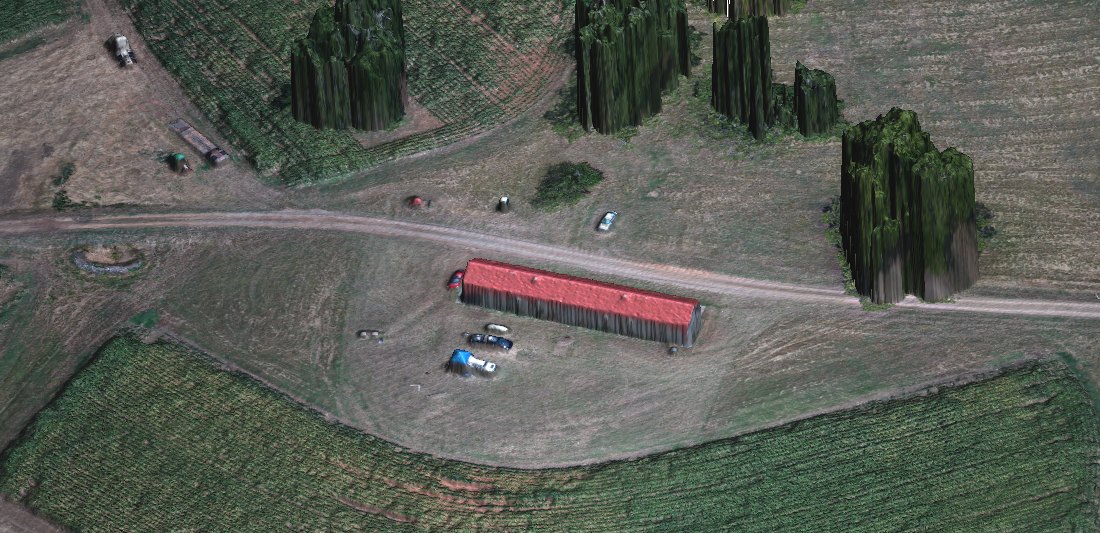
\includegraphics[width=\textwidth]{agisoft_detail}
  \\
  \tiny
  \textcolor{gray}{surface interpolated from points from SfM}
\end{center}

\end{column}
\end{columns}

\end{frame}


%%%%%%%%%%%%%%%%%%%%%%%%%%%%%%%%%%%%%%%%%%%%%%%%%%%%%%%%%%%%%%%%%%%%%
\begin{frame}{Acknowledgements}

\begin{columns}
\begin{column}{0.48\textwidth}

\begin{block}{Datasets}
\footnotesize
Lidar and UAV Structure from Motion (SfM) data for
\href{http://ncsu-osgeorel.github.io/uav-lidar-analytics-course/}%
  {GIS595/MEA792: UAV/lidar Data Analytics} course

\smallskip

Nantahala NF, NC: Forest Leaf Structure, Terrain and Hydrophysiology.
% Lidar data acquisition and processing completed
% by the National Center for Airborne Laser Mapping (\href{http://www.ncalm.org}{NCALM}).
% NCALM funding provided by NSF's Division of Earth Sciences, Instrumentation and Facilities Program.
% EAR-1043051.
Obtained from \href{http://www.opentopography.org/}{OpenTopography}.
\url{http://dx.doi.org/10.5069/G9HT2M76}
\end{block}

\end{column}
\begin{column}{0.47\textwidth}

\begin{center}
  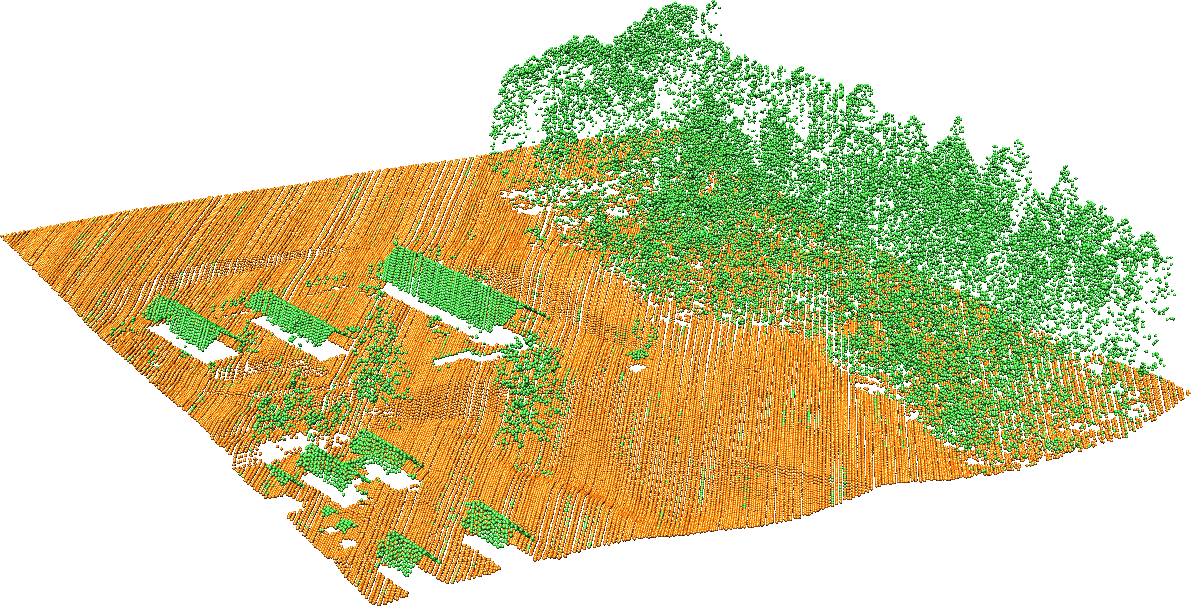
\includegraphics[width=\textwidth]{lidar_secref_3d}
\end{center}

\end{column}
\end{columns}

\end{frame}


%%%%%%%%%%%%%%%%%%%%%%%%%%%%%%%%%%%%%%%%%%%%%%%%%%%%%%%%%%%%%%%%%%%%%
\begin{frame}{Free, libre and open source}

\begin{columns}
\begin{column}{0.4\textwidth}

Scripts and code I'm writing

\begin{itemize}
  \item review
  \item re-usable
  \begin{itemize}
  \item by other people
  \item by future myself
  \end{itemize}
\end{itemize}

Software I'm using

\begin{itemize}
  \item driven by needs of users
  \item longevity
  \begin{itemize}
  \item learn now, use forever
  \item GRASS GIS: over 30 years of development
  \end{itemize}
\end{itemize}

\end{column}
\begin{column}{0.3\textwidth}

\begin{center}
  
\includegraphics[width=\textwidth]{logos/open_science}
  \\
  \tiny
  \textcolor{gray}{Open Science Logo, Greg Emmerich, CC-BY-SA-2.0}
\end{center}

\end{column}
\end{columns}

\end{frame}


%%%%%%%%%%%%%%%%%%%%%%%%%%%%%%%%%%%%%%%%%%%%%%%%%%%%%%%%%%%%%%%%%%%%%
\begin{frame}{GRASS GIS}

\begin{columns}
\begin{column}{0.4\textwidth}

\begin{itemize}
  \item universal scientific and processing platform
  \begin{itemize}
  \item GUI, CLI, Python API
  \item from small laptops to supercomputers
  \end{itemize}
  \item lidar processing included
  \item data size and type challenges
\end{itemize}

\begin{center}

\includegraphics[width=0.3\textwidth]{logos/grass_gis}
\end{center}

\end{column}
\begin{column}{0.55\textwidth}

\begin{center}
  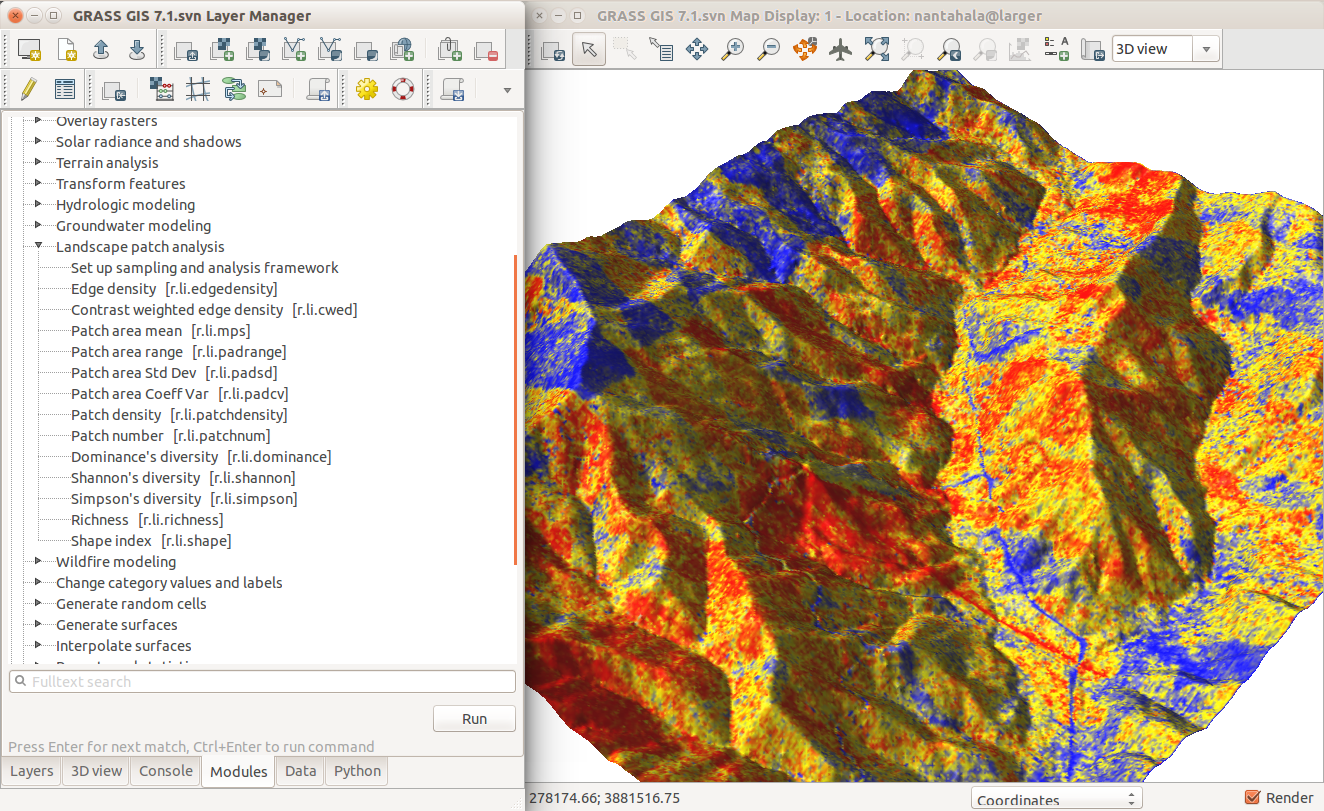
\includegraphics[width=\textwidth]{grass/count_and_modules}
\end{center}

\end{column}
\end{columns}

\end{frame}


%%%%%%%%%%%%%%%%%%%%%%%%%%%%%%%%%%%%%%%%%%%%%%%%%%%%%%%%%%%%%%%%%%%%%
\begin{frame}{Acknowledgements}

\begin{columns}
\begin{column}{0.6\textwidth}

\begin{block}{Software}
Presented functionality is work done by Vaclav Petras, Markus Metz, and the GRASS development team.

\bigskip

Thanks to users for feedback and testing, especially to
Douglas Newcomb, Helena Mitasova, Markus Neteler, Laura Belica, and William Hargrove.
\end{block}

\end{column}
\begin{column}{0.3\textwidth}

\begin{center}
  
\includegraphics[width=\textwidth]{logos/grass_gis}
\end{center}

\end{column}
\end{columns}

\end{frame}


%%%%%%%%%%%%%%%%%%%%%%%%%%%%%%%%%%%%%%%%%%%%%%%%%%%%%%%%%%%%%%%%%%%%%
\begin{frame}{Workflow overview}

\includegraphics[width=\textwidth]%
    {grass/workflow}

\end{frame}

%%%%%%%%%%%%%%%%%%%%%%%%%%%%%%%%%%%%%%%%%%%%%%%%%%%%%%%%%%%%%%%%%%%%%
\begin{frame}{Binning as 2D histogram}

\begin{columns}
\begin{column}{0.4\textwidth}

 \begin{itemize}
  \item counts number of points in cell
\end{itemize}

\end{column}
\begin{column}{0.45\textwidth}

\begin{center}
  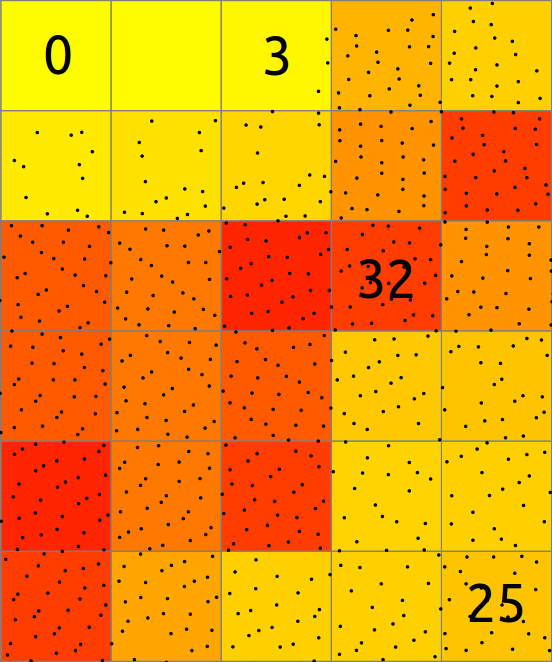
\includegraphics[width=0.75\textwidth]{features/binning_count}
\end{center}

\end{column}
\end{columns}

\end{frame}

%%%%%%%%%%%%%%%%%%%%%%%%%%%%%%%%%%%%%%%%%%%%%%%%%%%%%%%%%%%%%%%%%%%%%
\begin{frame}{Binning points to raster}

\begin{columns}
\begin{column}{0.4\textwidth}

 \begin{itemize}
  \item \gmodule{r.in.lidar} (import and analysis)
  \item statistics of point counts, height and intensity
  \begin{itemize}
    \item n, min, max, sum
    \item mean, range, skewness, \ldots
  \end{itemize}
\end{itemize}

\end{column}
\begin{column}{0.45\textwidth}

\begin{center}
  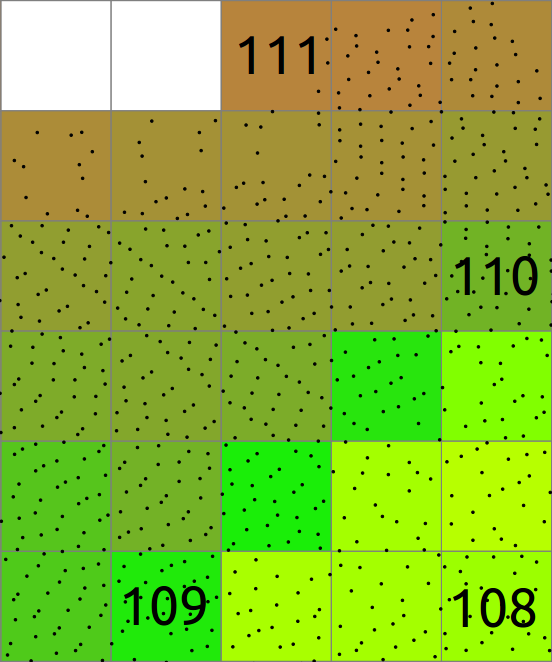
\includegraphics[width=0.75\textwidth]{features/binning_mean}
\end{center}

\end{column}
\end{columns}

\end{frame}


%%%%%%%%%%%%%%%%%%%%%%%%%%%%%%%%%%%%%%%%%%%%%%%%%%%%%%%%%%%%%%%%%%%%%
\begin{frame}{Practical functions}

\begin{columns}
\begin{column}{0.45\textwidth}

 \begin{itemize}
  \item analytical and practical functions in \gmodule{r.in.lidar}
  %\begin{itemize}
  \item read multiple tiles as one
    \begin{itemize}
    \item no merging
    \item 0.5 billion points in 90 files in minutes
    \end{itemize}
  %\end{itemize}
\end{itemize}

\end{column}
\begin{column}{0.54\textwidth}

\begin{center}
  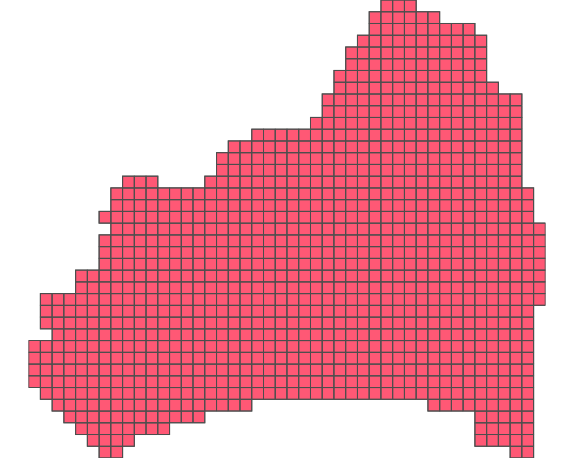
\includegraphics[width=\textwidth]{features/tiles}
\end{center}

\end{column}
\end{columns}

\end{frame}

%%%%%%%%%%%%%%%%%%%%%%%%%%%%%%%%%%%%%%%%%%%%%%%%%%%%%%%%%%%%%%%%%%%%%
\begin{frame}{Filtering points}

\begin{columns}
\begin{column}{0.38\textwidth}

 \begin{itemize}
  \item filter points by
  \begin{itemize}
    \item range of Z
    \item return
    \item class
    \item \ldots
  \end{itemize}
  \item at the time of binning with \gmodule{r.in.lidar}
    \begin{itemize}
    \item minimal additional cost
    \end{itemize}
\end{itemize}

\end{column}
\begin{column}{0.6\textwidth}

\begin{center}
  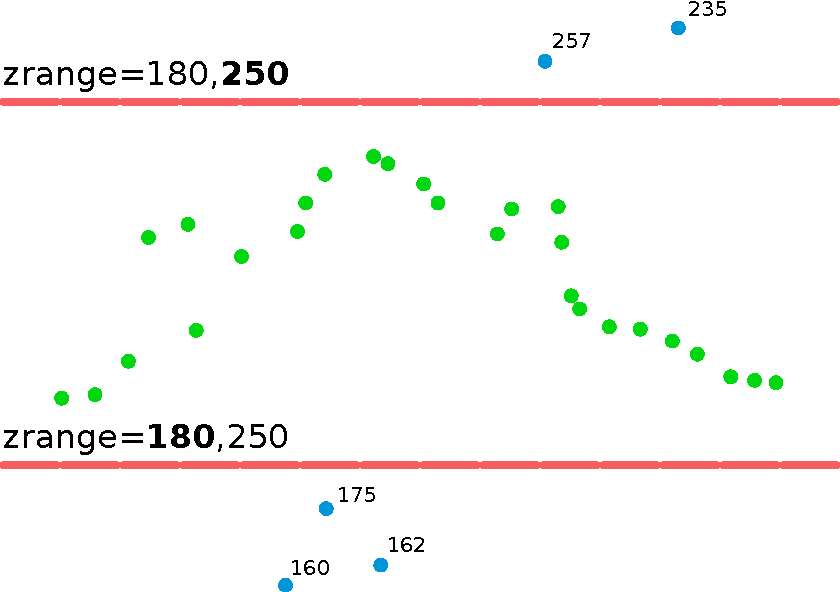
\includegraphics[width=0.75\textwidth]{features/zrange}
\end{center}

\end{column}
\end{columns}

\end{frame}

%%%%%%%%%%%%%%%%%%%%%%%%%%%%%%%%%%%%%%%%%%%%%%%%%%%%%%%%%%%%%%%%%%%%%
\begin{frame}{Height above a surface}

\begin{columns}
\begin{column}{0.4\textwidth}

\begin{itemize}
  \item new base raster feature in \gmodule{r.in.lidar}
  \item given surface $+$ points cloud\\
    $\longrightarrow$ height of features
\end{itemize}

\medskip

\begin{center}
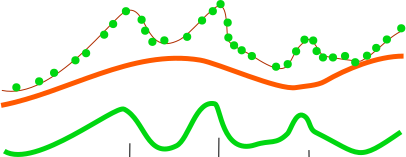
\includegraphics[width=\textwidth]{images/features/base_raster}
\end{center}

\begin{itemize}
  \item \small not limited by memory
\end{itemize}

\end{column}
\begin{column}{0.55\textwidth}

\begin{center}
  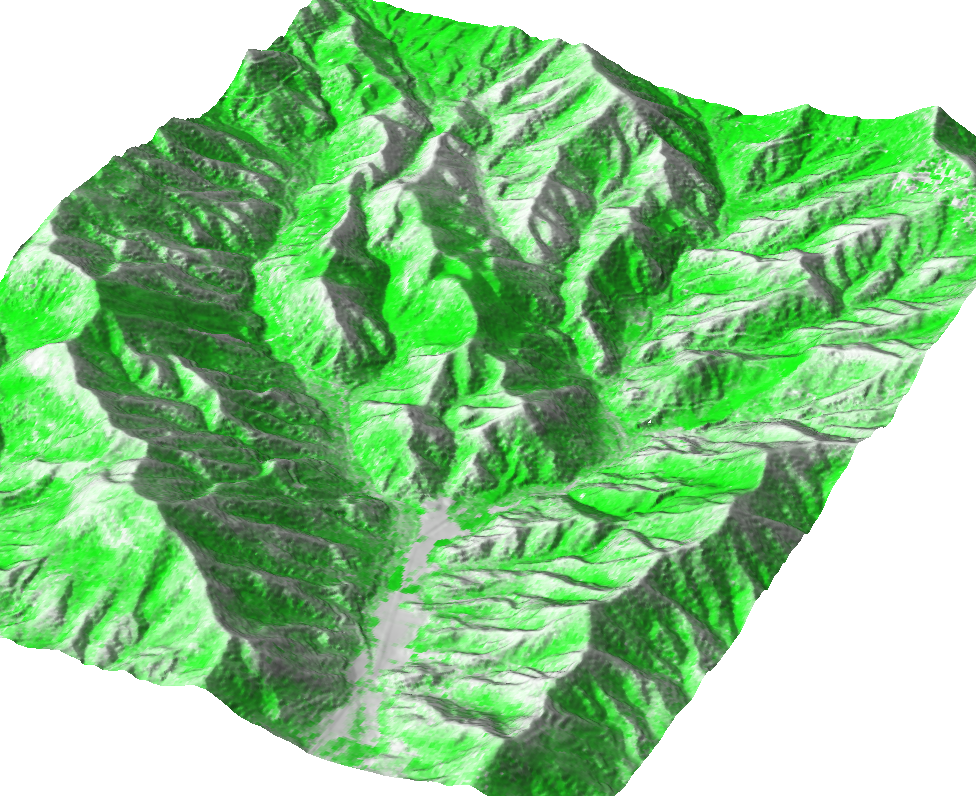
\includegraphics[width=\textwidth]{grass/max_height_10m_on_ground_from_neighbors_smaller_area_top}
\end{center}

\end{column}
\end{columns}

\end{frame}


%%%%%%%%%%%%%%%%%%%%%%%%%%%%%%%%%%%%%%%%%%%%%%%%%%%%%%%%%%%%%%%%%%%%%
\begin{frame}{Rasterize early}

\begin{columns}
\begin{column}{0.4\textwidth}

\begin{itemize}
  \item less cells then points
  \begin{itemize}
    \item 578 mil points (ground 30 mil)
    \item 15 mil cells in 8km\,$\times$\,7km at~resolution 2m
    \begin{itemize}
    \item faster to loop through
    \item less disk space
    \end{itemize}
  \end{itemize}
  \item raster
  \begin{itemize}
    \item natural spatial index
    \item that's what the algorithms use
  \end{itemize}
\end{itemize}

\end{column}
\begin{column}{0.45\textwidth}

\begin{center}
  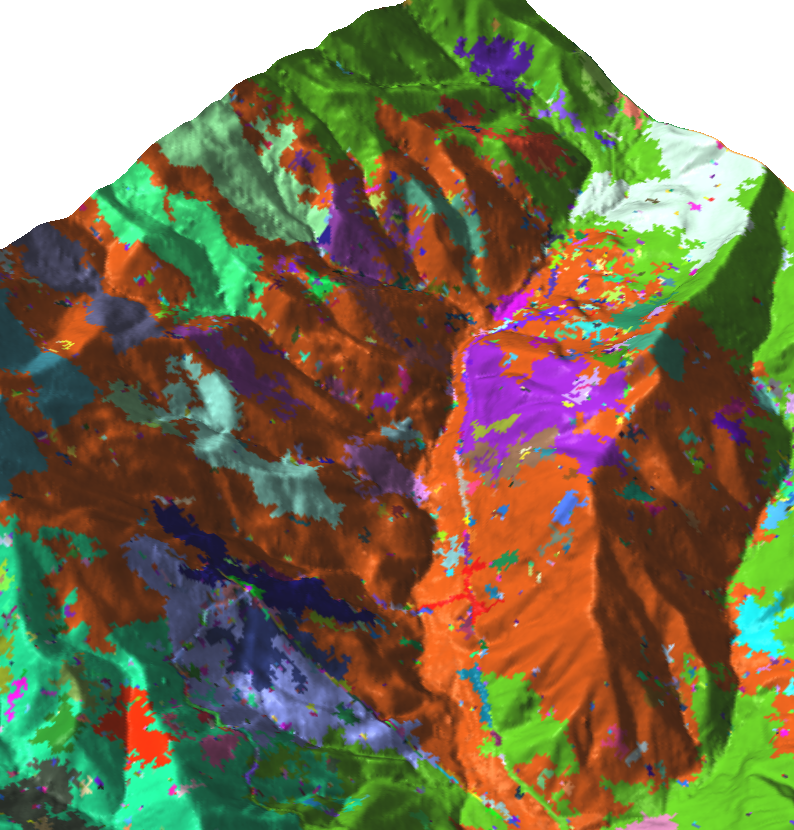
\includegraphics[width=0.75\textwidth]{grass/segment_on_counts}
  \\
  \tiny
  \textcolor{gray}{\gmodule{i.segment} on different point counts}
\end{center}

\end{column}
\end{columns}

\end{frame}

%%%%%%%%%%%%%%%%%%%%%%%%%%%%%%%%%%%%%%%%%%%%%%%%%%%%%%%%%%%%%%%%%%%%%
\begin{frame}{3D raster}

\begin{columns}
\begin{column}{0.38\textwidth}

\begin{itemize}
  \item stacked 2D rasters
  \item challenging to visualize
  \item same principles as in 2D
  \begin{itemize}
  \item e.g. 3D raster map algebra
  \end{itemize}
\end{itemize}

\end{column}
\begin{column}{0.5\textwidth}

\begin{center}
  \includegraphics<1>[width=\textwidth]{grass/raster_3d_cube}
  \includegraphics<2>[width=\textwidth]{grass/raster_3d_slices}
\end{center}

\end{column}
\end{columns}

% vis also possible using Tangible Landscape

\end{frame}


%%%%%%%%%%%%%%%%%%%%%%%%%%%%%%%%%%%%%%%%%%%%%%%%%%%%%%%%%%%%%%%%%%%%%
\begin{frame}{Binning points to 3D raster}

\begin{columns}
\begin{column}{0.28\textwidth}

\begin{itemize}
  \item \gmodule{r3.in.lidar}
  \item proportional count
  \begin{itemize}
    \item count per 3D cell relative to the count per vertical column
  \end{itemize}
  \item intensity can be used instead of count
\end{itemize}

\bigskip
\footnotesize
height reduction by base raster under development
\tiny
(analysis and space efficient)

\end{column}
\begin{column}{0.7\textwidth}

\begin{center}
  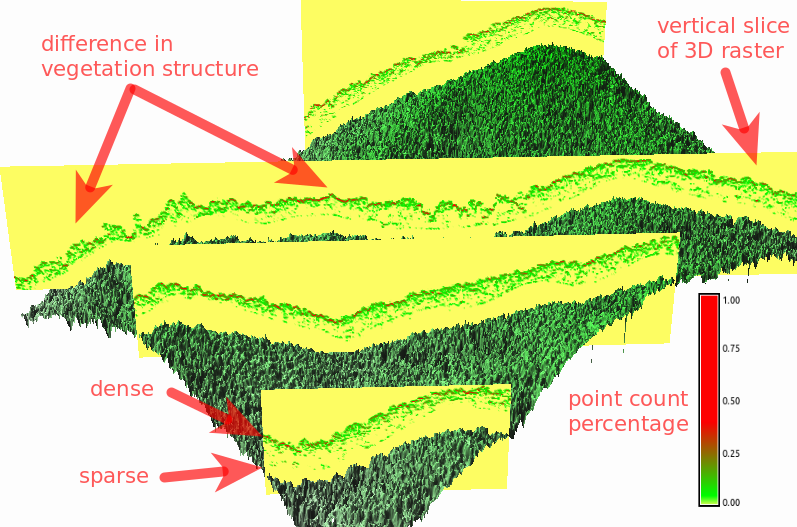
\includegraphics[width=\textwidth]{grass/red_green_3d_labels}
\end{center}

\end{column}
\end{columns}

\end{frame}


%%%%%%%%%%%%%%%%%%%%%%%%%%%%%%%%%%%%%%%%%%%%%%%%%%%%%%%%%%%%%%%%%%%%%
\begin{frame}{Decimation}

\begin{columns}
\begin{column}{0.58\textwidth}

\begin{itemize}
  \item \gmodule{v.in.lidar}
  \begin{itemize}
  \item filtering same as in \gmodule{r.in.lidar}
  \end{itemize}
  \item often more points than we need {\small\\ (research shows, Singh et al. 2015, Petras et al. 2016)}
  \item interpolation, clustering, \ldots\ are costly
  \item decimation~$\approx$~sampling
  \begin{itemize}
    \item fast count-based as effective as more advanced decimation
  \end{itemize}
\end{itemize}

\end{column}
\begin{column}{0.22\textwidth}

% TODO: UAV image

\begin{center}
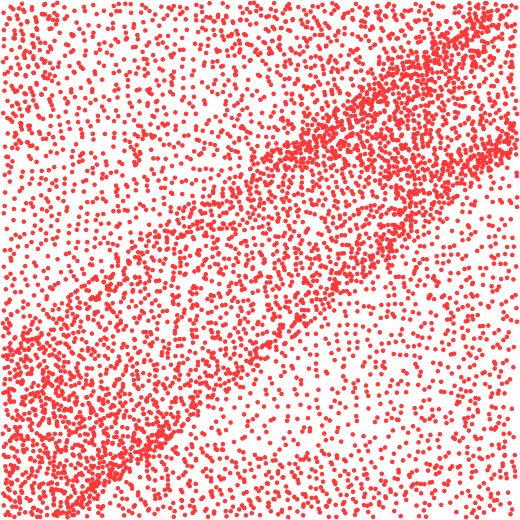
\includegraphics[width=\textwidth]{features/full}

\smallskip

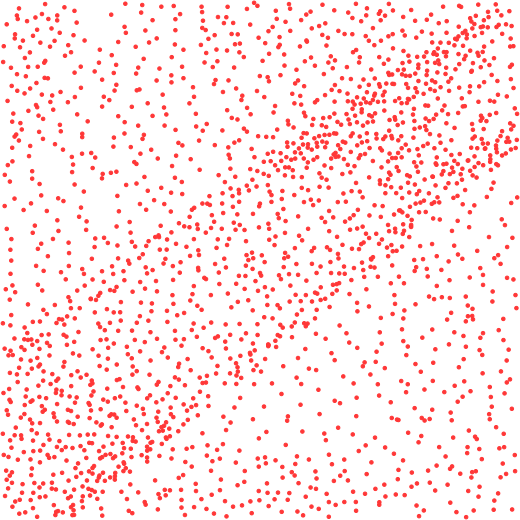
\includegraphics[width=\textwidth]{features/preserve}

\end{center}

\end{column}
\end{columns}

\end{frame}


%%%%%%%%%%%%%%%%%%%%%%%%%%%%%%%%%%%%%%%%%%%%%%%%%%%%%%%%%%%%%%%%%%%%%
\begin{frame}{Large point clouds}

\begin{columns}
\begin{column}{0.44\textwidth}

Rasters (binning of points)

\begin{itemize}
  \item trade-off: memory (RAM) or slow
  \item 64bit version
  \begin{itemize}
  \item \tiny your operating system may limit max memory
  \end{itemize}
\end{itemize}

\vspace{2.2ex}

\end{column}
\begin{column}{0.44\textwidth}

Vectors (points as points)

\begin{itemize}
  \item point cloud specific optimizations
  \begin{itemize}
  \item no IDs stored
  \item no attribute table
  \item no topology created
  \end{itemize}
\end{itemize}

\end{column}
\end{columns}

\begin{columns}
\begin{column}{0.44\textwidth}

\textcolor{gray}{
\footnotesize
Brunswick county: binning, $\approx$1050 files, $>9$~billion points % method=n, 13GB (40 thousand x 40 thousand cells, 5 ft res, >1.5 bil cells)
\\
Hyde county: binning, $\approx$950 files, $>4$~billion points, base elevation 5ft raster, 60ft height raster % 2.4 billion cells in base rast, about half water
\\
$\approx$0.5-3~hours, 1-13GB of memory \tiny (in-memory mode)
}

\end{column}
\begin{column}{0.44\textwidth}

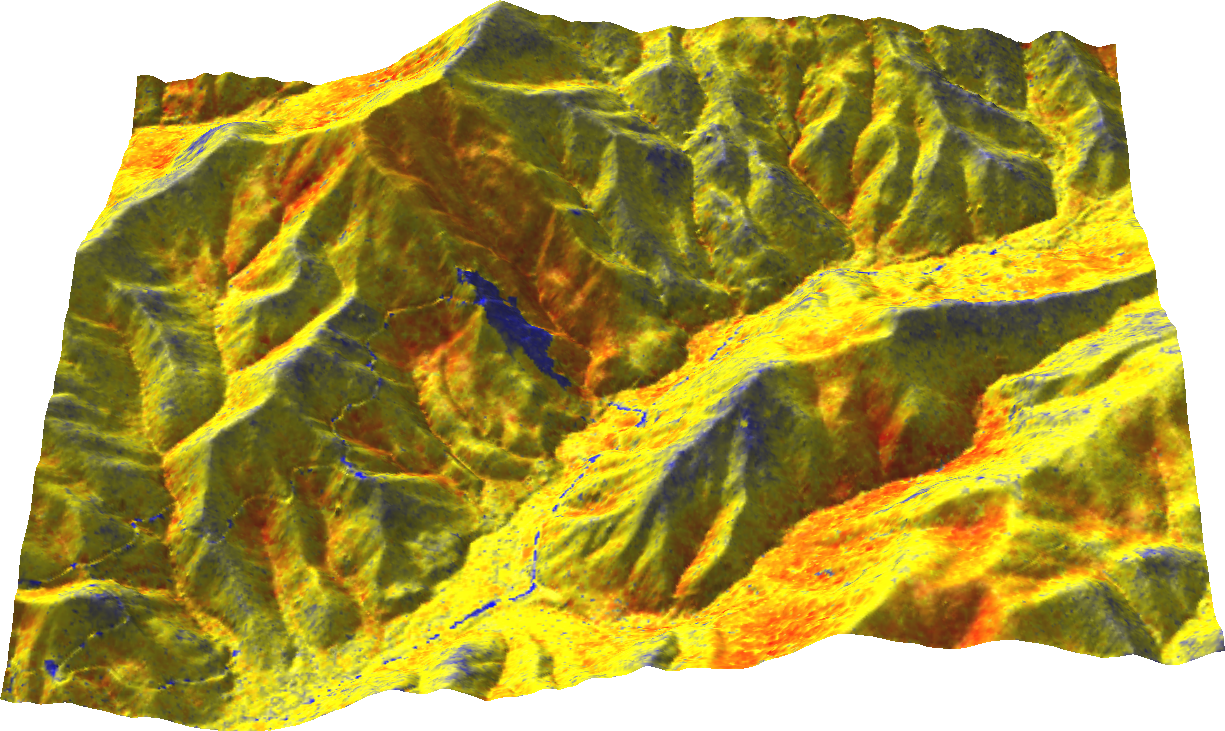
\includegraphics[width=\textwidth]{grass/range_on_ground_from_north}
%   \tiny
%   \textcolor{gray}{
%   range from \gmodule{r.in.lidar} on ground obtained
%   from \gmodule{v.in.lidar} followed by \gmodule{v.surf.rst}
%   }

\end{column}
\end{columns}

\end{frame}


%%%%%%%%%%%%%%%%%%%%%%%%%%%%%%%%%%%%%%%%%%%%%%%%%%%%%%%%%%%%%%%%%%%%%
\begin{frame}{Ground detection}

\begin{columns}
\begin{column}{0.28\textwidth}

\begin{itemize}
\item \gmodule{v.lidar.edgedetection}, \gmodule{v.lidar.growing}, \gmodule{v.lidar.correction}
\begin{itemize}
  \item uses returns
\end{itemize}

\item \amodule{v.lidar.mcc}
\begin{itemize}
  \item multiscale curvature based classification algorithm\footnotemark[1]
\end{itemize}

\end{itemize}

\end{column}
\begin{column}{0.7\textwidth}

\begin{center}
  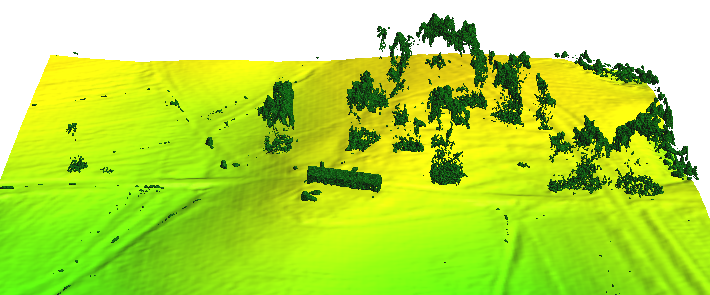
\includegraphics[width=\textwidth]{grass/mcc_default}
\end{center}

\end{column}
\end{columns}

\bigskip

% cannot use normal footnotes because they are limited to the column
\footnoterule
\footnotesize
\footnotemark[1]
Evans, J. S. \& Hudak, A. T. 2007: A Multiscale Curvature Algorithm for Classifying Discrete Return LiDAR in Forested Environments.
% IEEE TRANSACTIONS ON GEOSCIENCE AND REMOTE SENSING 45(4): 1029 - 1038.

\end{frame}


%%%%%%%%%%%%%%%%%%%%%%%%%%%%%%%%%%%%%%%%%%%%%%%%%%%%%%%%%%%%%%%%%%%%%
\begin{frame}{Sky-view factor}

\begin{itemize}
  \item \amodule{r.skyview} (percentage of visible sky)
\end{itemize}

\begin{center}
  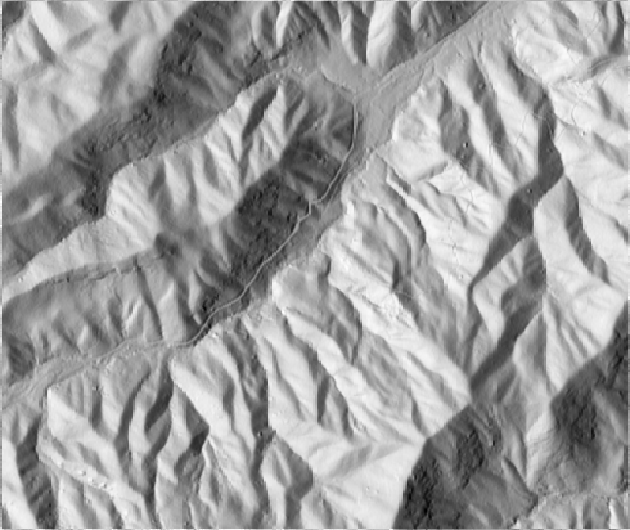
\includegraphics[width=0.45\textwidth]{vis/shade}
  ~
  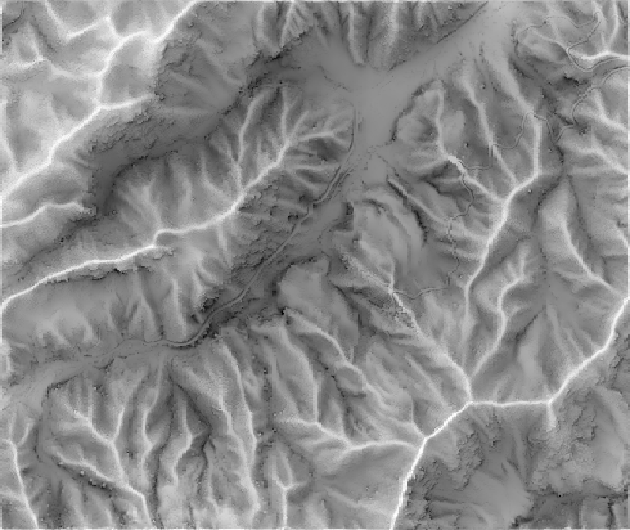
\includegraphics[width=0.45\textwidth]{vis/skyview_ridges}
  \\
  {\footnotesize comparison of shaded relief and sky-view factor}
  % 412*4 (1648) x 490*4 (1960)
\end{center}

\end{frame}


%%%%%%%%%%%%%%%%%%%%%%%%%%%%%%%%%%%%%%%%%%%%%%%%%%%%%%%%%%%%%%%%%%%%%
\begin{frame}{Local relief model (LRM)}

\begin{itemize}
  \item \amodule{r.local.relief} (micro-topography, features other than trend)
\end{itemize}

\begin{center}
  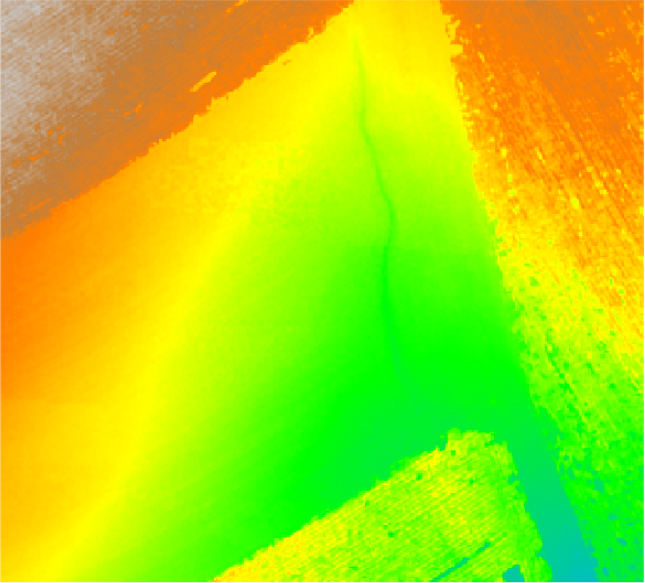
\includegraphics[width=0.4\textwidth]{vis/elevation}
  ~~
  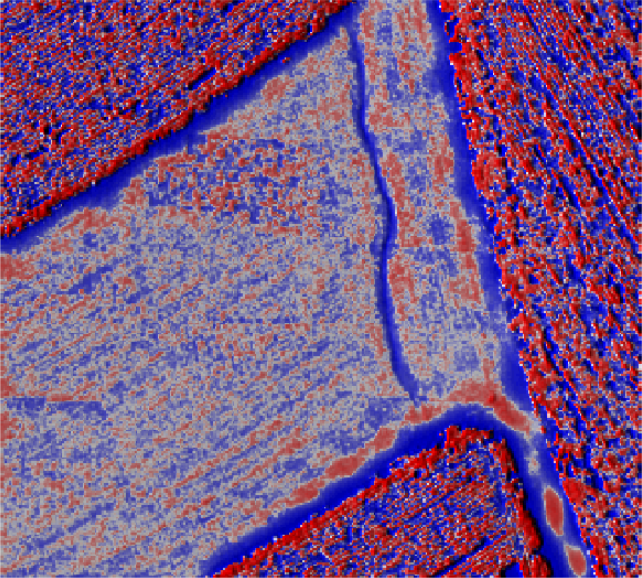
\includegraphics[width=0.4\textwidth]{vis/lrm}\\
  \footnotesize
  30-60cm wide, 30cm deep, 60m long gully (resolution 30cm)
  % 294 rows, 325 cols (88.2m x 97.5m)
\end{center}

\end{frame}


%%%%%%%%%%%%%%%%%%%%%%%%%%%%%%%%%%%%%%%%%%%%%%%%%%%%%%%%%%%%%%%%%%%%%
\begin{frame}{Landforms}

\begin{columns}
\begin{column}{0.3\textwidth}

\begin{itemize}
  \item \amodule{r.geomorphon}
  \item geomorphons - a new approach to classification of landform\footnotemark[1]
\end{itemize}

\footnotesize
\footnotemark[1]
Jasiewicz, J., Stepinski, T., 2013,
Geomorphons - a pattern recognition approach to classification and mapping of landforms, Geomorphology%
% vol. 182, 147-156 (DOI: 10.1016/j.geomorph.2012.11.005)

\end{column}
\begin{column}{0.68\textwidth}

\begin{center}
  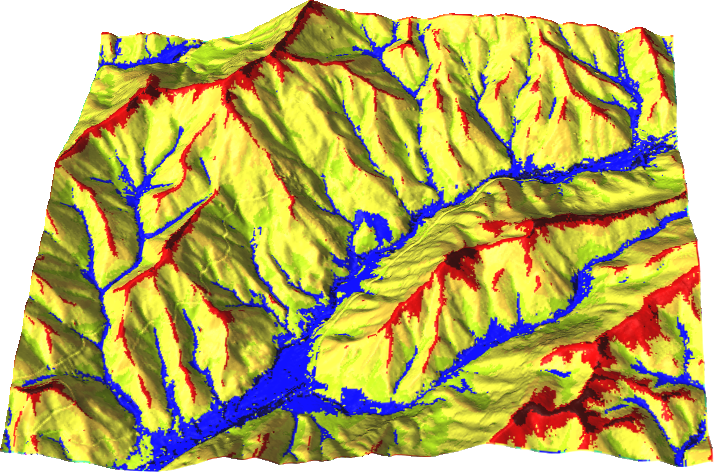
\includegraphics[width=\textwidth]{vis/geomorphon_3d}
\end{center}

\end{column}
\end{columns}

\end{frame}

%%%%%%%%%%%%%%%%%%%%%%%%%%%%%%%%%%%%%%%%%%%%%%%%%%%%%%%%%%%%%%%%%%%%%
\begin{frame}{Integration with PDAL}

\begin{columns}
\begin{column}{0.5\textwidth}

\begin{block}{PDAL}
 \begin{itemize}
  \item Point Data Abstraction Library
  \item formats besides LAS/LAZ
  \item algorithms, filters, decimations
 \end{itemize}
\end{block}

\begin{block}{Experimental integration}
 \begin{itemize}
  \item \module{v.in.pdal}
  \item reprojection during import
  \item ground filter
  \item compute height as a difference from ground
 \end{itemize}
\end{block}

\end{column}
\begin{column}{0.25\textwidth}

\begin{center}
  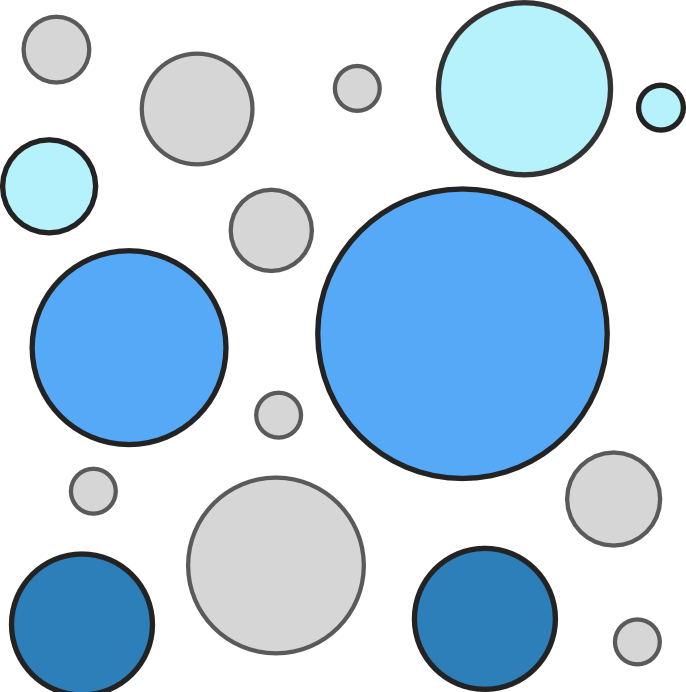
\includegraphics[width=\textwidth]{logos/pdal_bubbles}\\
  
\includegraphics[width=\textwidth]{logos/pdal_text}
\end{center}

\end{column}
\end{columns}

\end{frame}


%%%%%%%%%%%%%%%%%%%%%%%%%%%%%%%%%%%%%%%%%%%%%%%%%%%%%%%%%%%%%%%%%%%%%
\begin{frame}{}

% logo at the bottom can be moved down
\vspace*{0.05\textheight}

\begin{block}{Summary}
 \begin{itemize}
  \item rasterize early
  \item make use of existing methods for raster and vector processing
  \item 3D rasters, PDAL integration
  \item the plan for next 30 years driven by users
    -- \href{https://lists.osgeo.org/listinfo/grass-user}{grass-user mailing list}
 \end{itemize}
\end{block}

\bigskip
\centering

\begin{tabular}{clc}
\begin{minipage}{0.16\textwidth}

\includegraphics[width=\textwidth]{logos/grass_gis}
\end{minipage}
&
\begin{minipage}{0.4\textwidth}
\footnotesize
\href{https://grass.osgeo.org/download/}{%
Get GRASS GIS 7.1 development version at\\
\texttt{grass.osgeo.org/download}%
}

\bigskip

{
\footnotesize
Slides available at\\
\href{http://wenzeslaus.github.io/grass-lidar-talks/}%
  {\texttt{wenzeslaus.github.io/grass-lidar-talks}}
}

%\bigskip

{
\footnotesize
Paper in preparation:
\emph{Processing UAV and lidar point clouds in GRASS GIS}
}
\end{minipage}
&
\begin{minipage}{0.2\textwidth}

\includegraphics[width=\textwidth]{talks_qr}
\end{minipage}
\end{tabular}

\end{frame}


\end{document}
